\documentclass[a4paper,12pt]{article}
\usepackage[utf8]{inputenc}
\usepackage[T1]{fontenc}
\usepackage[french]{babel}
\usepackage{graphicx} % Pour inclure des images
\usepackage{hyperref} % Pour les liens hypertextes
\usepackage{amsmath} % Pour les équations
\usepackage{geometry} % Pour ajuster les marges
\geometry{margin=1in} % Définit les marges du document

\title{Guide de configuration de l'expérience d'usure et acquisition d'images avec GelSight}
\author{Antoine Boucher}
\date{Mars 2025}

\begin{document}

\maketitle

\tableofcontents

\section{Introduction}
L'objectif de ce guide est de détailler la mise en place de l'expérience d'usure ainsi que l'acquisition d'images avec le capteur \textbf{GelSight}. Ce document présente également, de manière innovante, la procédure de réalisation robotisée des tests d'usure. Grâce à un système robotisé contrôlé via la base de code, il est désormais possible de réaliser des tests précis et reproductibles en appliquant de manière automatisée des pressions et des cycles de mouvement sur des échantillons soigneusement préparés. Cette approche moderne vous positionne à la pointe de la recherche expérimentale, en alliant robustesse technologique et analyse fine des matériaux.

\section{Matériel requis}
Avant de commencer, assurez-vous d'avoir le matériel suivant :
\begin{itemize}
    \item \textbf{Plateforme d'usure} : Surface et matériaux à tester.
    \item \textbf{GelSight} : Capteur de mesure pour la prise d'images en haute résolution.
    \item \textbf{Éclairage contrôlé} : Lampe LED uniforme pour éviter les variations d’éclairage.
    \item \textbf{Caméra haute résolution} : Connectée à un ordinateur pour capturer les images.
    \item \textbf{PC avec logiciel d'acquisition} : Interface de contrôle pour le capteur et stockage des images.
    \item \textbf{Supports et fixations} : Pour stabiliser les échantillons et le capteur pendant l’expérience.
    \item \textbf{Système robotisé de tests d'usure} : Robot configuré pour réaliser les tests d'usure de manière automatisée.
\end{itemize}

\section{Création des échantillons}
Les échantillons doivent présenter des dimensions précises de 50 mm $\times$ 40 mm avec une épaisseur de 4 mm.

\subsection{Méthode 1 : Utilisation du moule pour matériaux en coulée liquide}
\begin{enumerate}
    \item \textbf{Préparation du moule} : Nettoyage et calibration du moule conformément aux paramètres définis dans le code.
    \item \textbf{Chargement du matériau liquide} : Injection homogène du matériau en état liquide dans la cavité du moule.
    \item \textbf{Solidification} : Activation d'un système de refroidissement pour assurer une solidification rapide et uniforme.
    \item \textbf{Démoulage} : Extraction automatique de l'échantillon formé, garantissant des dimensions précises de \textbf{50 mm $\times$ 40 mm} et une épaisseur de \textbf{4 mm}.
\end{enumerate}

\begin{figure}[h]
    \centering
    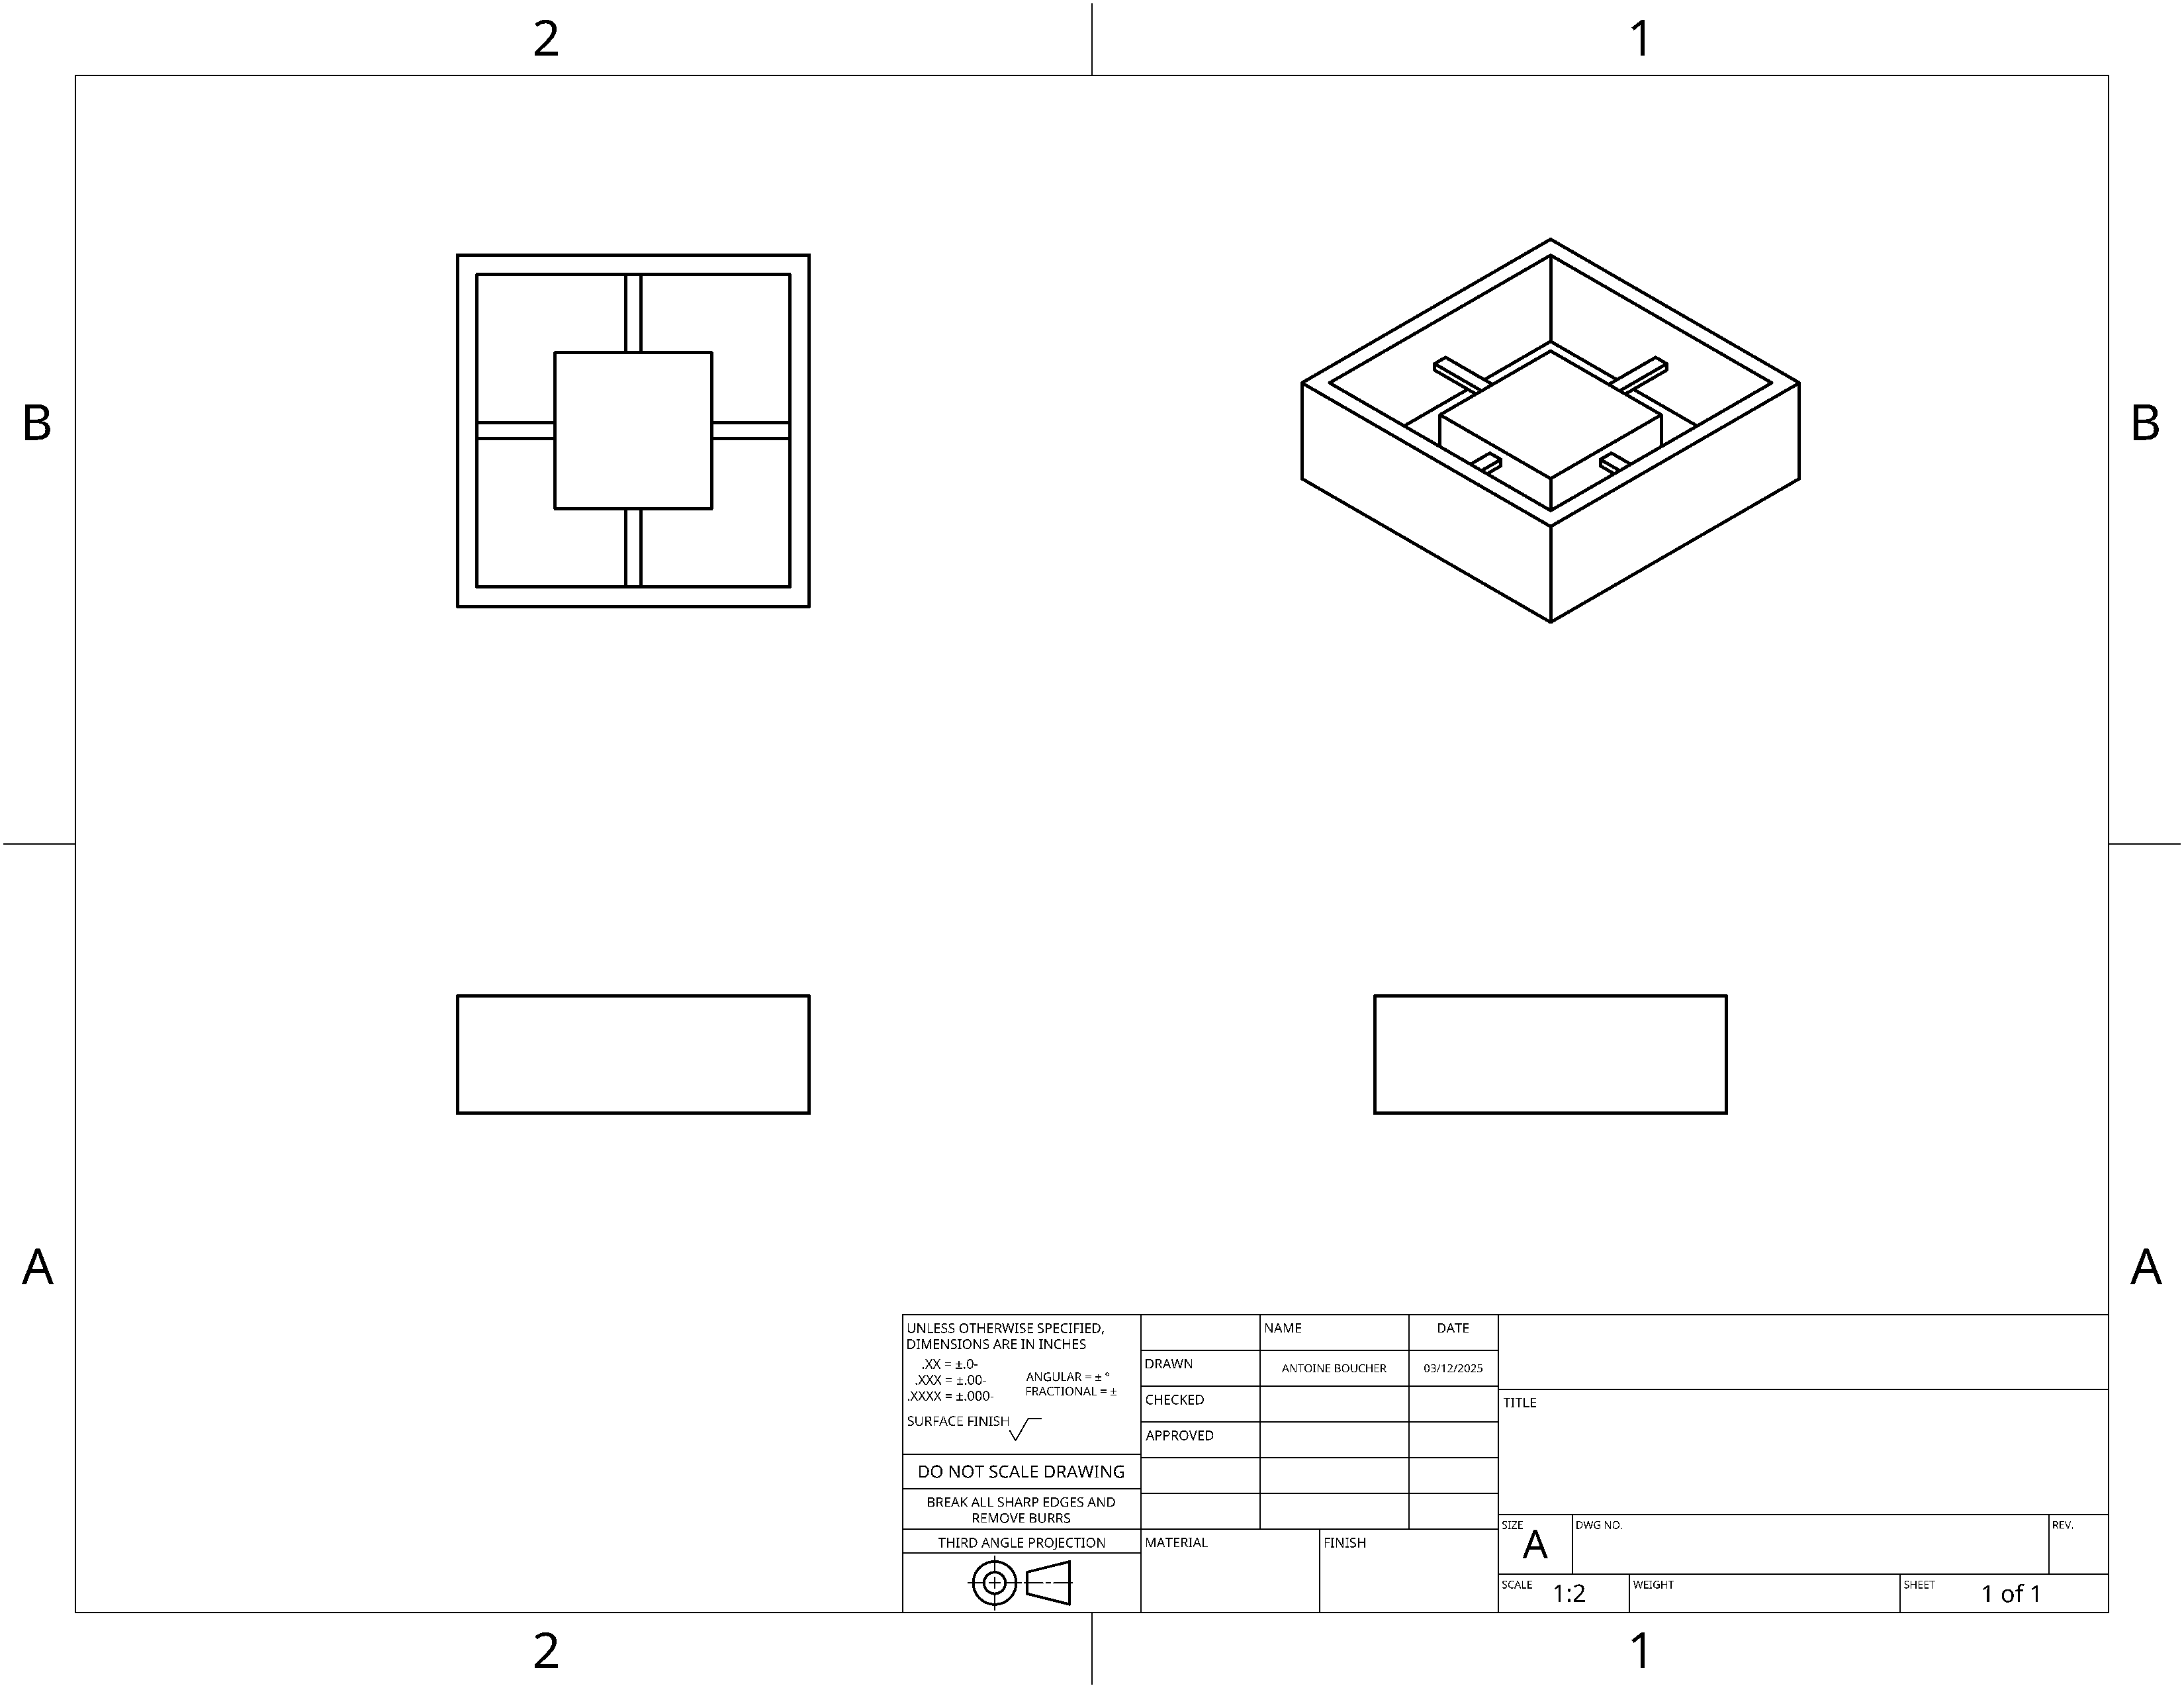
\includegraphics[width=0.5\linewidth]{Mold.png}
    \caption{Mold CAD}
    \label{fig:mold-cad}
\end{figure}

\subsection{Méthode 2 : Utilisation des modèles CAD pour la fabrication des échantillons}
\begin{enumerate}
    \item \textbf{Conception numérique} : Utilisation de modèles CAD intégrés dans la base de code pour définir les dimensions et la géométrie exacte de l'échantillon.
    \item \textbf{Préparation de l'outil de fabrication} : Transfert du modèle CAD vers le système robotisé, qui ajuste ses paramètres en fonction du design.
    \item \textbf{Fabrication additive ou soustractive} : Selon le matériau et la technologie disponible, le robot réalise l'échantillon en usinant ou en déposant le matériau couche par couche.
    \item \textbf{Contrôle qualité} : Vérification dimensionnelle automatisée pour s'assurer de la conformité des échantillons (50 mm $\times$ 40 mm et 4 mm d'épaisseur).
\end{enumerate}

\begin{figure}[h]
    \centering
    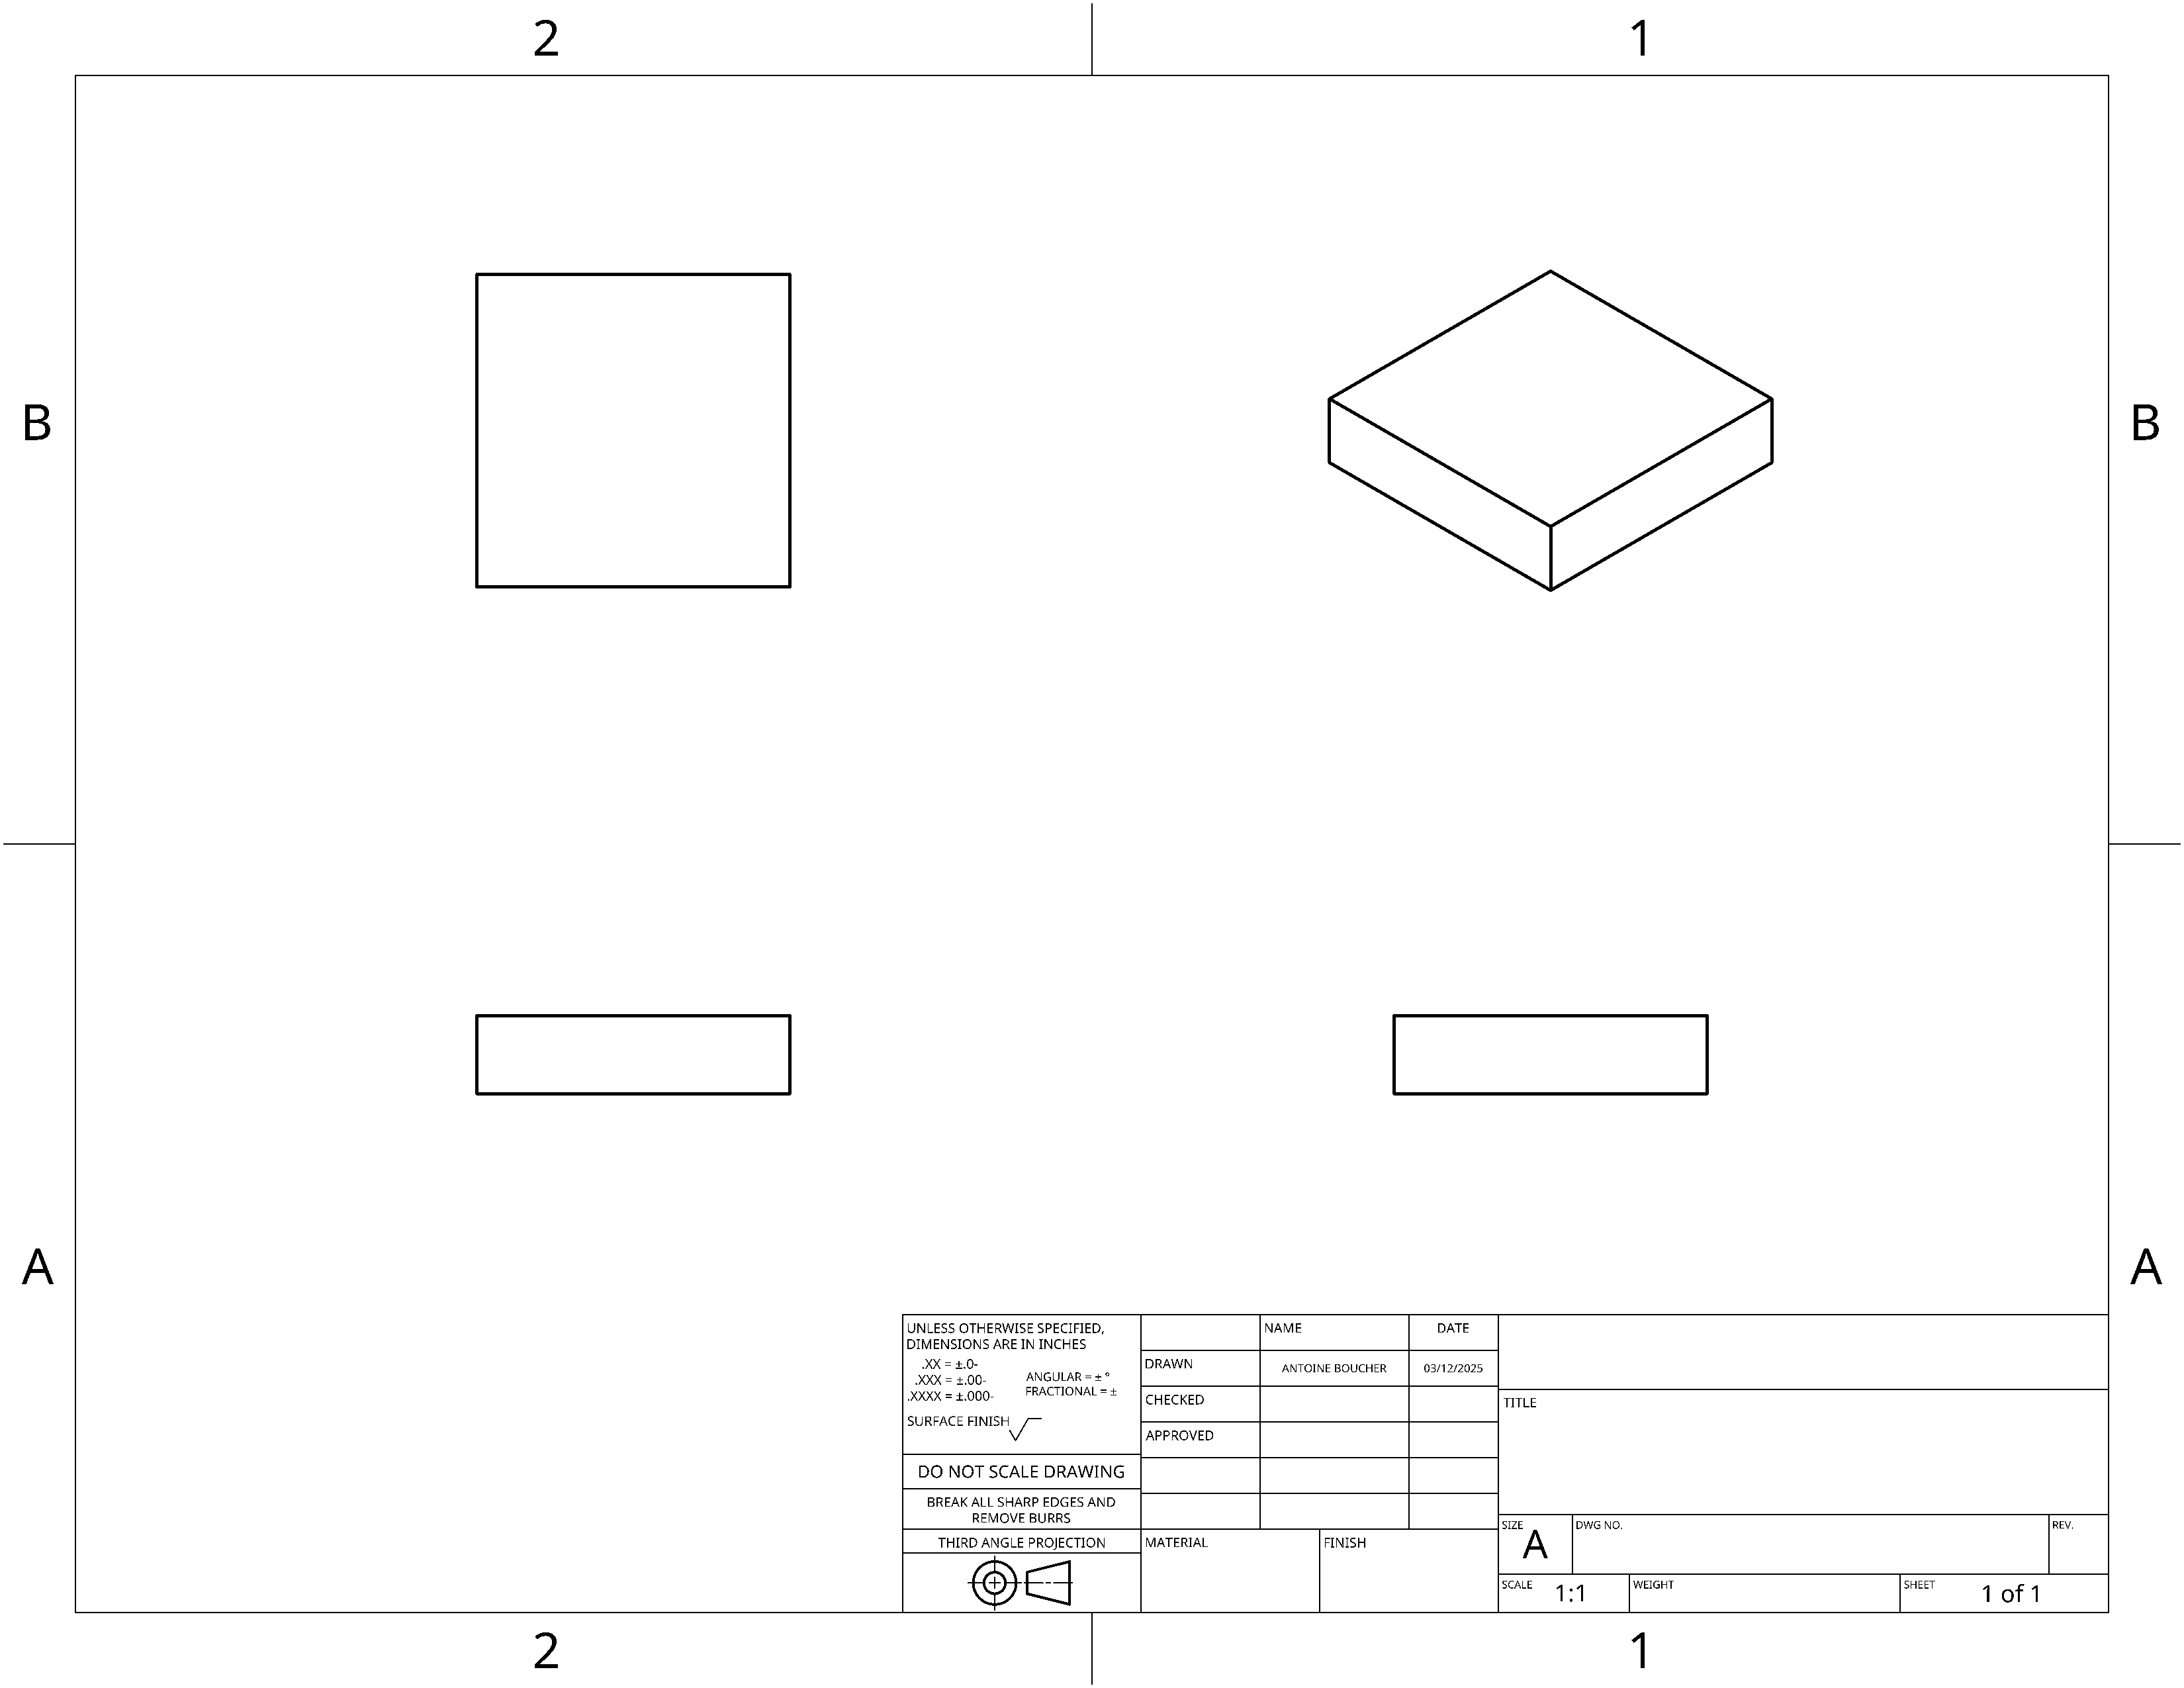
\includegraphics[width=0.5\linewidth]{Sample.png}
    \caption{Sample Mode}
    \label{fig:sample-mode}
\end{figure}

\section{Mise en place de l'expérience}
\subsection{Préparation des échantillons}
\begin{itemize}
    \item Sélectionner le matériau à tester (ex : acier, polymère, etc.).
    \item Nettoyer les surfaces pour éviter toute contamination.
    \item Fixer l’échantillon sur la plateforme d’usure à l’aide de supports stables.
\end{itemize}

\subsection{Assemblage du robot}
\subsubsection{Composants supplémentaires pour l'assemblage du robot}
\begin{itemize}
    \begin{figure}
        \centering
        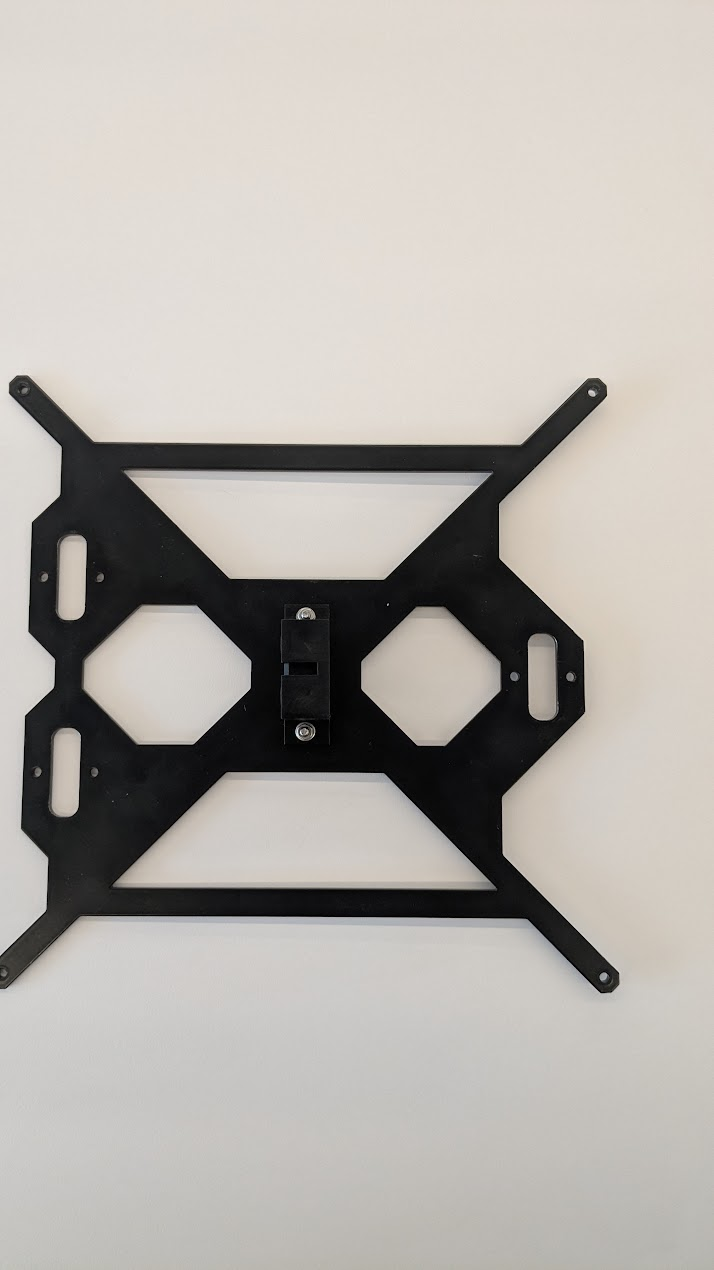
\includegraphics[width=0.5\linewidth]{image.png}
        \caption{Base}
        \label{fig:enter-label}
    \end{figure}
    \begin{figure}
        \centering
        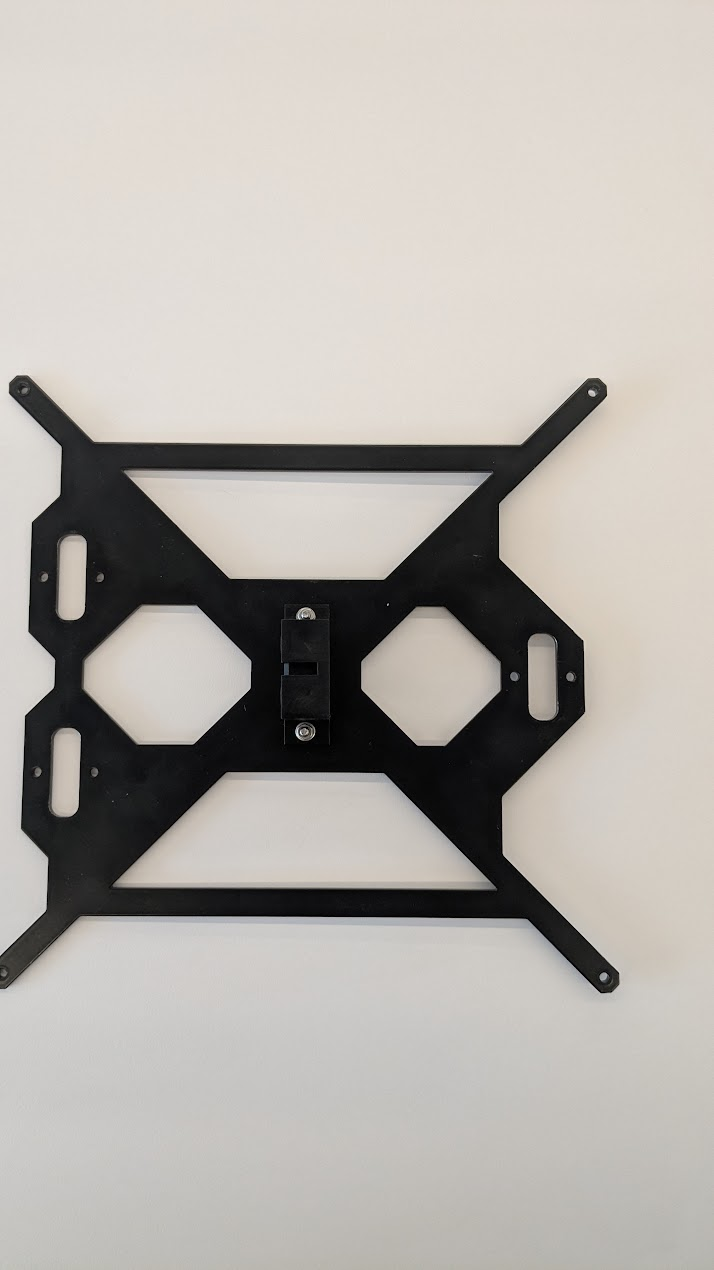
\includegraphics[width=0.5\linewidth]{image.png}
        \caption{Base}
        \label{fig:enter-label}
    \end{figure}
    \item \textbf{Arduino Mega 128} : Carte microcontrôleur pilotant l'ensemble du système.
    \begin{figure}
        \centering
        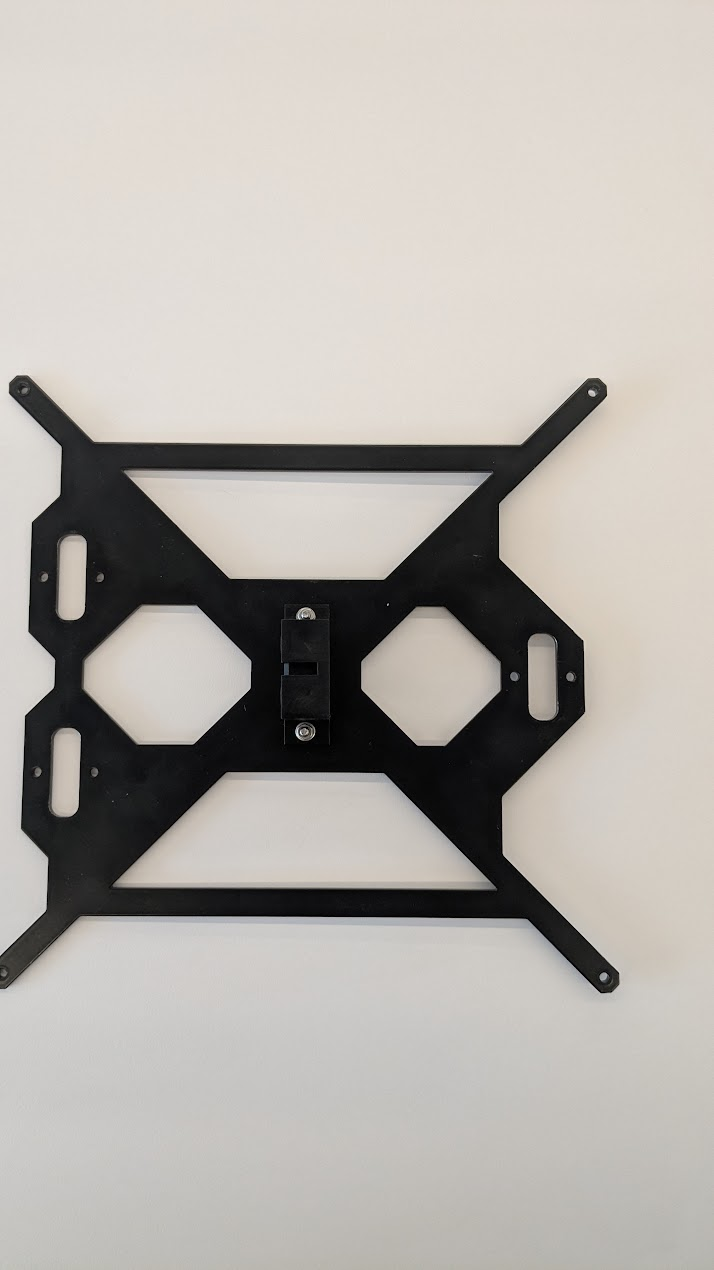
\includegraphics[width=0.5\linewidth]{image.png}
        \caption{Arduino}
        \label{fig:enter-label}
    \end{figure}
    \item \textbf{Stepper Motor Nema 17} : Moteur pas à pas de haute précision pour contrôler les déplacements.
    \item \textbf{Câblage et connecteurs dédiés} : Pour assurer une connexion stable entre le moteur et l'Arduino.
    \item \textbf{Alimentation 9V (batterie ou adaptateur)} : Source d'énergie fiable pour l'ensemble du circuit.
    \begin{figure}
        \centering
        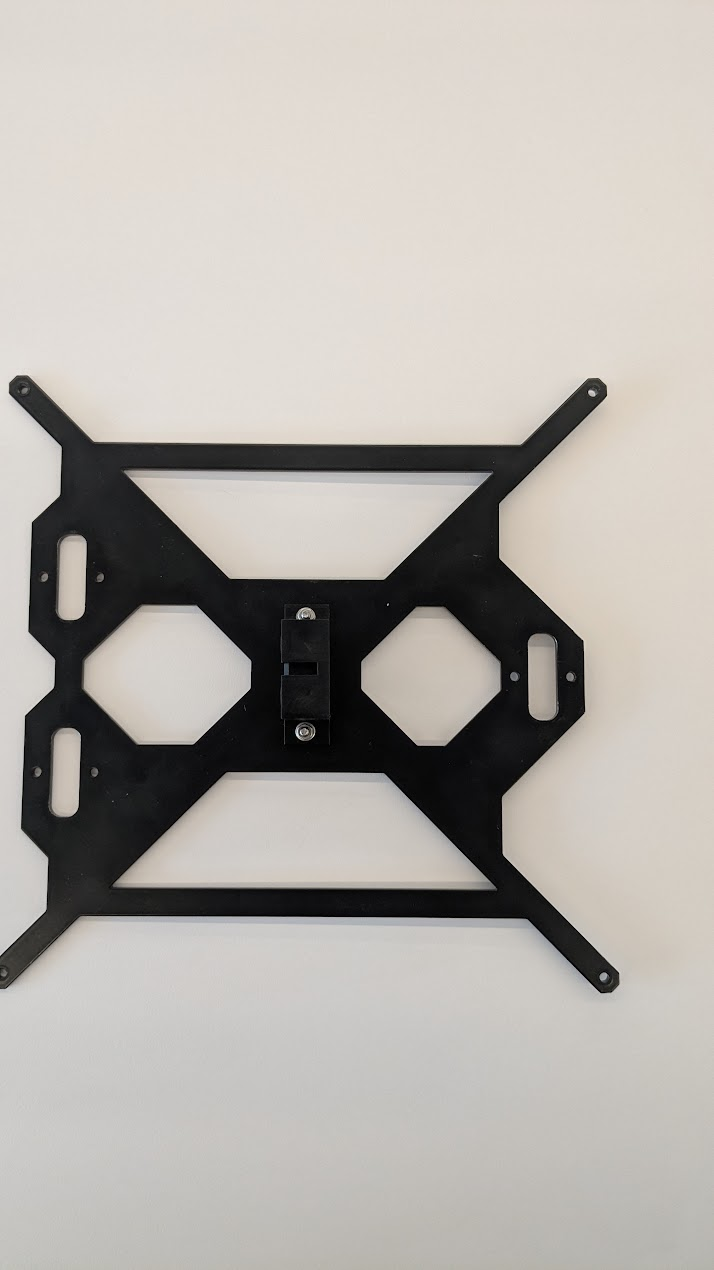
\includegraphics[width=0.5\linewidth]{image.png}
        \caption{Battery}
        \label{fig:enter-label}
    \end{figure}
    \item \textbf{Breadboard} : Pour le prototypage des circuits et connexions temporaires.
    \item \textbf{Logiciel Arduino sur PC} : Environnement de développement pour programmer et tester le robot.
    \item \textbf{USB vers cadre basé sur une courroie crantée} : Permet l'intégration d'un cadre de déplacement pour des mouvements précis.
    \begin{figure}
        \centering
        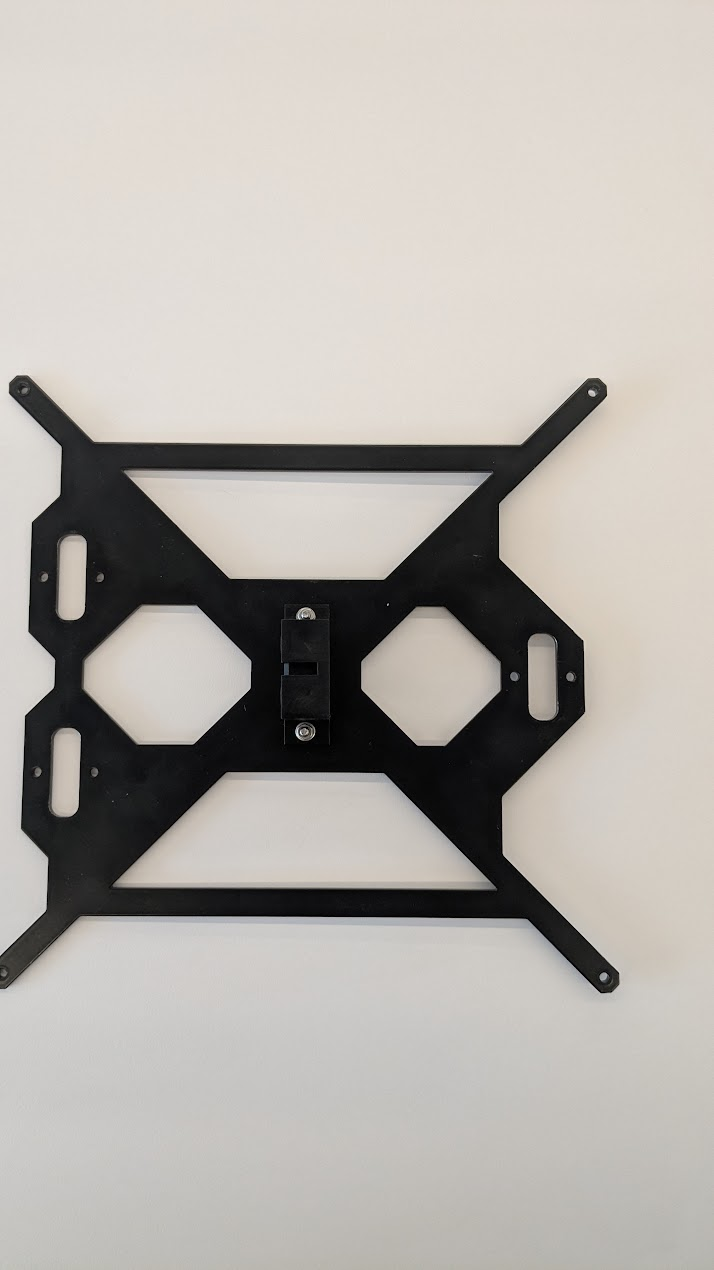
\includegraphics[width=0.5\linewidth]{image.png}
        \caption{Timing belt}
        \label{fig:enter-label}
    \end{figure}
\end{itemize}

\subsubsection{Assemblage et configuration du système robotisé}
\begin{enumerate}
    \item \textbf{Installation de l'Arduino} : Montez l'Arduino Mega 128 sur un support adapté et connectez-le à la breadboard.
    \item \textbf{Connexion du moteur} : Branchez le Stepper Motor Nema 17 à l'Arduino en utilisant les câbles et connecteurs appropriés.
    \item \textbf{Alimentation électrique} : Reliez l'alimentation 9V à l'Arduino et aux autres composants critiques.
    \item \textbf{Intégration du cadre de déplacement} : Fixez le cadre basé sur une courroie crantée et connectez-le via USB pour assurer une communication fluide.
    \item \textbf{Configuration logicielle} : Installez l'IDE Arduino sur votre PC et téléversez le code de contrôle sur la carte.
    \item \textbf{Tests et calibrations} : Effectuez des essais préliminaires pour valider les déplacements et ajuster les paramètres du robot.
\end{enumerate}

\subsection{Utilisation du robot pour les tests d'usure}
Le système robotisé est dédié à la réalisation des tests d'usure, et non à la fabrication des échantillons. Il permet de :
\begin{itemize}
    \item Appliquer de manière contrôlée la pression sur l'échantillon.
    \item Contrôler la vitesse et le déplacement pour simuler des conditions réelles d'usure.
    \item Répéter les cycles d'usure de manière précise et automatisée.
    \item Garantir la cohérence des tests en éliminant les variations humaines.
\end{itemize}
Le robot est programmé via la base de code pour ajuster automatiquement les paramètres expérimentaux, assurant ainsi la fiabilité et la reproductibilité des résultats.

\subsection{Calibration du capteur GelSight}
\begin{enumerate}
    \item Placer une surface de référence sous le capteur pour établir un point zéro.
    \item Ajuster l'éclairage pour éviter les reflets excessifs.
    \item Vérifier les paramètres du capteur dans le logiciel (résolution, contraste, etc.).
    \item Effectuer une capture d’image test pour valider la qualité.
\end{enumerate}

\subsection{Paramètres expérimentaux}
\begin{itemize}
    \item Définir la pression appliquée sur l’échantillon.
    \item Régler la vitesse du mouvement pour simuler l’usure réelle.
    \item Consigner la durée de chaque test et le nombre de cycles d’usure.
\end{itemize}

\subsection{Paramètres et Consommables Recommandés}

\begin{table}[h]
\centering
\caption{Recommended Settings for the GelSight BenchTop System using the Canon T3i camera and MP-E 65\,mm 1X--5X macro lens. 
For each magnification, the table shows horizontal and vertical field of view (FOV), recommended gel diameter, calibration target, and camera settings. 
\textit{Note: The Live View ISO setting increases brightness during live view and does not affect the captured images when the \texttt{Scan} button is pressed.}}
\label{tab:rec-settings}
\begin{tabular}{ccccccccc}
\hline
\textbf{Mag.} & \textbf{H FOV (mm)} & \textbf{V FOV (mm)} & \textbf{Gel Diam.} & \textbf{Target} & \textbf{Shutter} & \textbf{Aperture} & \textbf{ISO} & \textbf{Live V. ISO} \\
\hline
1X & 22.4 & 14.9 & 38\,mm (1.5")   & BGA D07 S10 & 0.5\,s & F 9.0 & 100 & 100 \\
2X & 14.2 & 9.4  & 38\,mm (1.5")   & BGA D03 S10 & 1\,s   & F 9.0 & 100 & 100 \\
3X & 11.0 & 7.3  & 32\,mm (1.25")  & BGA D03 S05 & 2\,s   & F 8.0 & 100 & 100 \\
4X & 5.5  & 3.7  & 32\,mm (1.25")  & BGA D03 S05 & 2\,s   & F 8.0 & 100 & 100 \\
5X & 4.0  & 2.9  & 29\,mm (1.125") & BGA D03 S05 & 2\,s   & F 8.0 & 100 & 100 \\
\hline
\end{tabular}
\end{table}


\subsubsection{Paramètres Recommandés}
Le guide utilisateur décrit les réglages optimaux pour le système GelSight Benchtop utilisant un appareil Canon T3i et un objectif macro MP-E 65mm 1X–5X. Pour chaque niveau de magnification, le guide détaille :
\begin{itemize}
  \item Le champ de vision horizontal et vertical.
  \item Le diamètre du gel recommandé.
  \item La cible de calibration.
  \item Les réglages de l'appareil photo.
\end{itemize}
\noindent Remarque : Le réglage ISO en mode \texttt{Live View} augmente la luminosité pendant la prévisualisation, sans affecter l'image finale lors de l'appui sur le bouton \texttt{Scan}.

\subsubsection{Consommables Recommandés}
Pour une utilisation optimale du système, il est conseillé de disposer des consommables suivants :
\begin{itemize}
  \item Lingettes jetables sans peluches (McMaster-Carr part 7089T31) pour nettoyer le verre.
  \item Alcool isopropylique (91\%) en vaporisateur pour le nettoyage.
  \item Ruban adhésif double-face 3M VHB 2" (McMaster-Carr part 76665A89) pour créer des fixations et nettoyer le côté réfléchissant du gel.
  \item Plaques de verre pour supporter les échantillons (ex. : disque de verre de 2.5" de diamètre et 1/4" d'épaisseur, McMaster-Carr part 8477K78).
\end{itemize}

\subsection{Avant de Prendre des Mesures}
\begin{itemize}
  \item Créez un dossier (par exemple, nommé \texttt{Scans}) sur votre disque dur où vous disposez des droits de lecture et écriture.
  \item Lors du premier lancement de GSCapture, définissez le chemin d'accès de la bibliothèque via l'option \texttt{Paths} dans le menu \texttt{File}.
  \item Si vous utilisez également le logiciel MountainsMap pour l'analyse, désactivez la prévisualisation dans Windows Explorer afin d'éviter les problèmes de performance.
\end{itemize}

\subsection{Procédure de Prise de Mesures et Calibration Avancée}
\begin{enumerate}
  \item \textbf{Démarrage du Programme} : Double-cliquez sur l'exécutable \texttt{GSCapture}. Le programme se charge en mode \textit{Library}.
  \item \textbf{Connexion au Matériel} : Connectez-vous au capteur via \texttt{Device $\rightarrow$ Connect}. Vérifiez que la caméra est alimentée et que deux câbles USB sont connectés (un pour la caméra et un pour l'électronique).
  \item \textbf{Définition du Set de Mesures} : Cliquez sur \texttt{New Set} pour créer un nouvel ensemble de mesures.
  \item \textbf{Mode Capture et Réglages} : Ajustez les paramètres de l'appareil (vitesse, ouverture, ISO), sélectionnez l'éclairage, et utilisez \texttt{Live View} pour la mise au point. Choisissez entre \texttt{Single Image} ou \texttt{Scan} selon vos besoins.
  \item \textbf{Nommer et Lancer la Capture} : Entrez le nom du fichier et cliquez sur \texttt{Scan}. Chaque capture crée un dossier contenant un fichier \texttt{scan.yaml}.
  \item \textbf{Mode Calibration} : Ouvrez un dossier de scan ou le fichier \texttt{scan.yaml}, puis cliquez sur \texttt{Calibrate} pour accéder aux outils de calibration.
  \item \textbf{Sélection du Préréglage} : Choisissez le préréglage BGA approprié pour la calibration.
  \item \textbf{Processus de Calibration} :
  \begin{enumerate}
    \item Sélectionnez l'outil \texttt{Circle}.
    \item Choisissez deux (ou plusieurs) cercles adjacents centrés sur les billes.
    \item Cliquez sur \texttt{Extrapolate} pour calculer les positions.
  \end{enumerate}
  \item \textbf{Ajustement Fin} : Zoomez sur l'image et ajustez la position des cercles dans les coins de l'image. Cliquez sur \texttt{Update} après chaque ajustement. Utilisez l'option \texttt{Resize} pour modifier la taille des cercles si nécessaire.
  \item \textbf{Enregistrement} : Une fois l'alignement validé, cliquez sur \texttt{Save}.
  \item \textbf{Calcul du Modèle} : Sélectionnez les fichiers de calibration sauvegardés (généralement quatre fichiers BGA) ainsi que le fichier de référence \texttt{Glass Flat}. Entrez un nom pour le modèle et cliquez sur \texttt{Compute} (le modèle sera sauvegardé par défaut sous \texttt{model.yaml}).
\end{enumerate}

\subsection{Capture et Génération de Modèles 3D}
\begin{enumerate}
  \item Après le calcul du modèle, cliquez sur le bouton \texttt{Capture} pour scanner la surface.
  \item Sélectionnez le canal LED souhaité et activez le mode \texttt{Live View} pour ajuster la mise au point.
  \item Cliquez sur le bouton \texttt{10X} pour une focalisation fine.
  \item Entrez le nom du fichier et cliquez sur \texttt{Scan} pour capturer toutes les chaînes LED.
  \item Une fois le scan terminé, sélectionnez le dossier correspondant et choisissez \texttt{Generate 3D} dans le menu \texttt{File}.
  \item Dans la fenêtre de génération 3D, configurez l'algorithme, le nom du fichier et le niveau de \texttt{Detrend} désiré, puis cliquez sur \texttt{Process Scan}.
  \item Lorsque le fichier TMD est généré, double-cliquez dessus pour afficher la représentation 3D.
\end{enumerate}

\subsection{Outils de Traitement 3D (Optionnels)}
\begin{itemize}
  \item Utilisez le menu déroulant \texttt{Light Direction} pour modifier la direction de la lumière.
  \item Décochez \texttt{Color Height} pour obtenir une image 3D en niveaux de gris.
  \item Pour recadrer l'image 3D, sélectionnez l'outil \texttt{Rectangle} et délimitez la zone d'intérêt.
  \item Expérimentez avec différents niveaux de \texttt{Detrend} pour ajuster la planéité de l'image 3D, puis cliquez sur \texttt{Compute 3D Model} pour visualiser les effets.
\end{itemize}

\section{Procédure d'acquisition d'images}
\subsection{Positionnement du capteur}
\begin{itemize}
    \item Placer le capteur GelSight perpendiculairement à la surface d'usure.
    \item Vérifier l’alignement pour éviter toute ombre parasite.
    \item Maintenir une distance constante entre le capteur et l’échantillon.
\end{itemize}

\subsection{Prise des images}
\begin{enumerate}
    \item Lancer le logiciel d’acquisition et connecter le capteur.
    \item Régler les paramètres d’exposition et de balance des blancs.
    \item Capturer une image avant l’usure pour servir de référence.
    \item Réaliser des captures d’images à intervalles réguliers pendant l'expérience.
    \item Sauvegarder les images dans un format sans perte (ex : \texttt{.png}).
\end{enumerate}

\subsection{Stockage et organisation des fichiers}
\begin{itemize}
    \item Créer une structure de dossiers organisée (\texttt{expérience\_01/}, \texttt{expérience\_02/}, etc.).
    \item Nommer les fichiers de manière explicite (\texttt{avant\_usure.png}, \texttt{après\_10\_cycles.png}).
    \item Utiliser un script Python pour automatiser la sauvegarde et l’archivage.
\end{itemize}

\section{Intégration et synchronisation des systèmes}
Afin de garantir une coordination parfaite entre l'acquisition d'images et les tests d'usure robotisés, il est essentiel d'établir une synchronisation rigoureuse.

\subsection{Synchronisation des opérations}
\begin{itemize}
    \item \textbf{Déclenchement synchronisé} : Le logiciel de contrôle lance l'acquisition d'images exactement lorsque le robot atteint la position de test prédéfinie.
    \item \textbf{Communication en temps réel} : Utilisation d'un protocole (USB ou réseau local) pour assurer que les commandes et captures se déroulent simultanément.
    \item \textbf{Gestion des délais} : Intégration de temporisations précises pour éviter tout décalage entre le mouvement du robot et l'enregistrement des images.
\end{itemize}

\subsection{Automatisation via scripts et logiciels dédiés}
\begin{enumerate}
    \item Développer un script Python ou un programme sur l'IDE Arduino qui orchestre les différentes phases du test.
    \item Implémenter des boucles de contrôle pour vérifier en continu l'état du robot et du capteur.
    \item Enregistrer les données et images avec un horodatage pour faciliter l'analyse ultérieure.
\end{enumerate}

\section{Maintenance, sécurité et évolutivité}
La robustesse de l'expérience repose sur une maintenance régulière et une approche sécurisée et évolutive du système.

\subsection{Maintenance préventive}
\begin{itemize}
    \item Vérifier périodiquement les connexions électriques et mécaniques.
    \item Nettoyer et calibrer régulièrement le capteur GelSight pour garantir une qualité d'image optimale.
    \item Mettre à jour le code de contrôle pour bénéficier des dernières améliorations.
\end{itemize}

\subsection{Sécurité et gestion des risques}
\begin{itemize}
    \item Installer des dispositifs de sécurité (arrêts d'urgence, capteurs de surcharge) pour prévenir les accidents.
    \item Assurer une ventilation adéquate et un espace de travail organisé afin de minimiser les risques.
\end{itemize}

\subsection{Évolutivité du système}
\begin{itemize}
    \item Prévoir des interfaces modulaires pour intégrer de nouveaux capteurs ou modules robotisés.
    \item Mettre en place une documentation technique détaillée pour faciliter les mises à jour futures.
    \item Encourager le retour d'expérience afin d'orienter les améliorations et innovations.
\end{itemize}

\section{Perspectives d'amélioration et conclusion}
\subsection{Axes d'amélioration potentiels}
\begin{itemize}
    \item \textbf{Intelligence artificielle} : Intégrer des algorithmes de traitement d'images pour analyser automatiquement l'usure et identifier les zones critiques.
    \item \textbf{Rétroaction en temps réel} : Développer un système de monitoring permettant d'ajuster les paramètres expérimentaux en fonction des observations instantanées.
    \item \textbf{Extension des tests} : Adapter le système pour tester une gamme plus large de matériaux et simuler divers environnements d'usure.
\end{itemize}

\subsection{Conclusion}
En combinant l'expertise en acquisition d'images du capteur GelSight et l'automatisation des tests via un système robotisé, ce guide présente une approche innovante et fiable pour l'étude de l'usure des matériaux. Cette solution, à la fois flexible et évolutive, vous positionne résolument dans l'avenir de la recherche expérimentale. Continuez à innover et à explorer de nouvelles pistes pour enrichir et perfectionner vos protocoles de tests.

\end{document}
